\textbackslash{}chapter\{Lagrangian Dynamics\}
\textbackslash{}label\{ch:3\}

3.1
The principle of d'Alembert
by \textbackslash{}delta r\textbackslash{}alpha  has no effect. Furthermore, summing over all particles is just a sum
of terms all equal to zero. Thus the fact that the expression is equal to zero is
obviously true. What is not so obvious (yet) is why this particular formulation
is of any value.
We will begin by expressing d'Alembert's principle in Cartesian coordinates
and then transforming to generalized coordinates. For N particles there are
n = 3N Cartesian coordinates, and we can express d'Alembert's principle in
scalar form as
n

i=1

F ext
-$\textbackslash{}dot p$i

\textbackslash{}delta $\textbackslash{}xi$ = 0.
(3.3)
If there are n Cartesian coordinates and k constraints, we can (in principle)
express the problem in terms of n -k generalized coordinates. The transformation equations are
x1 = x1(q1, q2, . . . , qn-k, t)
x2 = x2(q1, q2, . . . , qn-k, t)
...
xn = xn(q1, q2, . . . , qn-k, t).
Note that although there are n Cartesian coordinates $\textbackslash{}xi$ there are only n -k
generalized coordinates because each constraint reduces by one the number of
degrees of freedom and hence the number of generalized coordinates.
The quantity \textbackslash{}delta ri in (3.2) or \textbackslash{}delta $\textbackslash{}xi$ in (3.3) is a virtual displacement. According
to Equation (1.9),
\textbackslash{}delta $\textbackslash{}xi$ =
n-k

j=1
\textbackslash{}partial $\textbackslash{}xi$
\textbackslash{}partial qj
\textbackslash{}delta qj.
Therefore, the first term in d'Alembert's principle can be written

F ext
\textbackslash{}delta $\textbackslash{}xi$ =

F ext
⎛
⎝
j
\textbackslash{}partial $\textbackslash{}xi$
\textbackslash{}partial qj
\textbackslash{}delta qj
⎞
⎠=

i,j

F ext
\textbackslash{}partial $\textbackslash{}xi$
\textbackslash{}partial qj

\textbackslash{}delta qj =

j
Qj\textbackslash{}delta qj.
The last quantity is the ``virtual work.'' (It is the work done during the virtual
displacement. See Section 1.6.)
Next consider the other term in d'Alembert's principle, namely $\textbackslash{}dot p$i\textbackslash{}delta $\textbackslash{}xi$:
n

$\textbackslash{}dot p$i\textbackslash{}delta $\textbackslash{}xi$ =
n

$\textbackslash{}dot p$i
n-k

j
\textbackslash{}partial $\textbackslash{}xi$
\textbackslash{}partial qj
\textbackslash{}delta qj =
n

mi $\textbackslash{}ddot x$i
n-k

j
\textbackslash{}partial $\textbackslash{}xi$
\textbackslash{}partial qj
\textbackslash{}delta qj,

where we assumed the masses of the particles are constant. But,
dt

mi $\textbackslash{}dot x$i
\textbackslash{}partial $\textbackslash{}xi$
\textbackslash{}partial qj

= mi $\textbackslash{}ddot x$i
\textbackslash{}partial $\textbackslash{}xi$
\textbackslash{}partial qj
+ mi $\textbackslash{}dot x$i
dt
\textbackslash{}partial $\textbackslash{}xi$
\textbackslash{}partial qj
.
Recall Equation (1.7):
\textbackslash{}partial $\textbackslash{}xi$
\textbackslash{}partial qj
= \textbackslash{}partial $\textbackslash{}dot x$i
\textbackslash{}partial $\textbackslash{}dot q$j
,
and note further that the last term of the previous equation involves the
expression
dt
\textbackslash{}partial $\textbackslash{}xi$
\textbackslash{}partial qj
= \textbackslash{}partial vi
\textbackslash{}partial qj
= \textbackslash{}partial $\textbackslash{}dot x$i
\textbackslash{}partial qj
.
Consequently,

$\textbackslash{}dot p$i\textbackslash{}delta $\textbackslash{}xi$ =

i,j

dt

mi $\textbackslash{}dot x$i
\textbackslash{}partial $\textbackslash{}xi$
\textbackslash{}partial qj

-mi $\textbackslash{}dot x$i
\textbackslash{}partial $\textbackslash{}dot x$i
\textbackslash{}partial qj

\textbackslash{}delta qj,
=

i,j

dt

mi $\textbackslash{}dot x$i
\textbackslash{}partial $\textbackslash{}dot x$i
\textbackslash{}partial $\textbackslash{}dot q$j

-mi $\textbackslash{}dot x$i
\textbackslash{}partial $\textbackslash{}dot x$i
\textbackslash{}partial qj

\textbackslash{}delta qj.
But
\textbackslash{}partial T
\textbackslash{}partial qj
=
\textbackslash{}partial
\textbackslash{}partial qj

2mi $\textbackslash{}dot x$2

=


$\textbackslash{}dot x$i
\textbackslash{}partial $\textbackslash{}dot x$i
\textbackslash{}partial qj

,
and
\textbackslash{}partial T
\textbackslash{}partial $\textbackslash{}dot q$j
=
\textbackslash{}partial
\textbackslash{}partial $\textbackslash{}dot q$j

2mi $\textbackslash{}dot x$2

=


$\textbackslash{}dot x$i
\textbackslash{}partial $\textbackslash{}dot x$i
\textbackslash{}partial $\textbackslash{}dot q$j

,
so finally,

$\textbackslash{}dot p$i\textbackslash{}delta $\textbackslash{}xi$ =

j

dt
\textbackslash{}partial T
\textbackslash{}partial $\textbackslash{}dot q$j
-\textbackslash{}partial T
\textbackslash{}partial qj

\textbackslash{}delta qj,
and d'Alembert's principle reads
n

i=1

F ext
-$\textbackslash{}dot p$i

\textbackslash{}delta $\textbackslash{}xi$ =

j
Qj\textbackslash{}delta qj -

j

dt
\textbackslash{}partial T
\textbackslash{}partial $\textbackslash{}dot q$j
-\textbackslash{}partial T
\textbackslash{}partial qj

\textbackslash{}delta qj = 0,
0 =

j

Qj -d
dt
\textbackslash{}partial T
\textbackslash{}partial $\textbackslash{}dot q$j
+ \textbackslash{}partial T
\textbackslash{}partial qj

\textbackslash{}delta qj.

3.2
Hamilton's principle
Since the \textbackslash{}delta qj are independent, each term in the series must individually be
equal to zero, so
dt
\textbackslash{}partial T
\textbackslash{}partial $\textbackslash{}dot q$j
-\textbackslash{}partial T
\textbackslash{}partial qj
= Qj.
(3.4)
This is called the Nielsen form of Lagrange's equations. Thus we have derived
Lagrange's equations in terms of generalized forces and kinetic energy. If the
generalized forces are derivable from a potential that is independent of the
generalized velocities, we can write Qj = -\textbackslash{}partial V/\textbackslash{}partial qj, and consequently,
dt
\textbackslash{}partial T
\textbackslash{}partial $\textbackslash{}dot q$j
-\textbackslash{}partial T
\textbackslash{}partial qj
= -\textbackslash{}partial V
\textbackslash{}partial qj
.
That is,
dt
\textbackslash{}partial (T -V )
\textbackslash{}partial $\textbackslash{}dot q$j
-\textbackslash{}partial (T -V )
\textbackslash{}partial qj
= 0.
This yields the familiar form of Lagrange's equations:
dt
\textbackslash{}partial L
\textbackslash{}partial $\textbackslash{}dot q$j
-\textbackslash{}partial L
\textbackslash{}partial qj
= 0.
(3.5)
Equations (3.4) and (3.5) are equivalent expressions for Lagrange's equations.
\begin{exercise}
Exercise 3.1 Using the Nielsen form, determine the equation of motion
for a mass m connected to a spring of constant k.
\end{exercise}

\begin{exercise}
Exercise 3.2 Using the Nielsen form, determine the equations of motion
for a planet in orbit around the Sun. (Answer: m$\textbackslash{}ddot r$ -mr $\textbackslash{}dot\textbackslash{}$theta 2 = -GMm
r2
and
mr $\textbackslash{}ddot \textbackslash{}theta$  + 2m$\textbackslash{}dot r$ $\textbackslash{}dot\textbackslash{}$theta  = 0.)
3.2 Hamilton's principle
A mechanical system composed of N particles can be described by n = 3N
Cartesian coordinates. All of these coordinates may not be independent. If
there are k equations of constraint, the number of independent coordinates is
n-k. The set of values for all the coordinates at a given instant of time is called
the configuration of the system at that time. That is, the configuration is given
by \{q1, q2, . . . , qn-k\}. We shall assume that all of the generalized coordinates
can be varied independently. (When we consider how to determine the forces

of constraint, we will formulate the problem in terms of generalized coordinates that are not all independent. But, for now, keep in mind that all the qis
are independent.)
Recall that the system can be represented as a point in the (n -k) dimensional space called configuration space. As time goes on, the coordinates of
the particles will change in a continuous manner and the point describing the
system will move in configuration space. As the system goes from an initial
configuration to a final configuration this point traces out a path or trajectory
in configuration space. Obviously there are infinitely many paths between the
initial point and the final point. We know, however, that a mechanical system
always takes a particular path between these two points. What is special about
the path actually taken? Hamilton's principle answers this question. It states
that the path taken by a system is the path that minimizes the ``action.'' The
action of a mechanical system is defined as the line integral
I =
t2
t1
Ldt,
(3.6)
where
L = L(q1, q2, . . . , qn-k; $\textbackslash{}dot q$1, $\textbackslash{}dot q$2, . . . , $\textbackslash{}dot q$n-k; t),
is the Lagrangian of the system and the limits on the integral, t1 and t2, are
the initial and final times for the process. Hamilton's principle tells us that
the system behaves in such a way as to minimize this integral. Therefore, the
variation of the integral is zero. In equation form, Hamilton's principle is
\textbackslash{}delta
t2
t1
Ldt = 0.
(3.7)
To interpret this relation, imagine a configuration space and an initial and final
\begin{figure}[h]
\centering
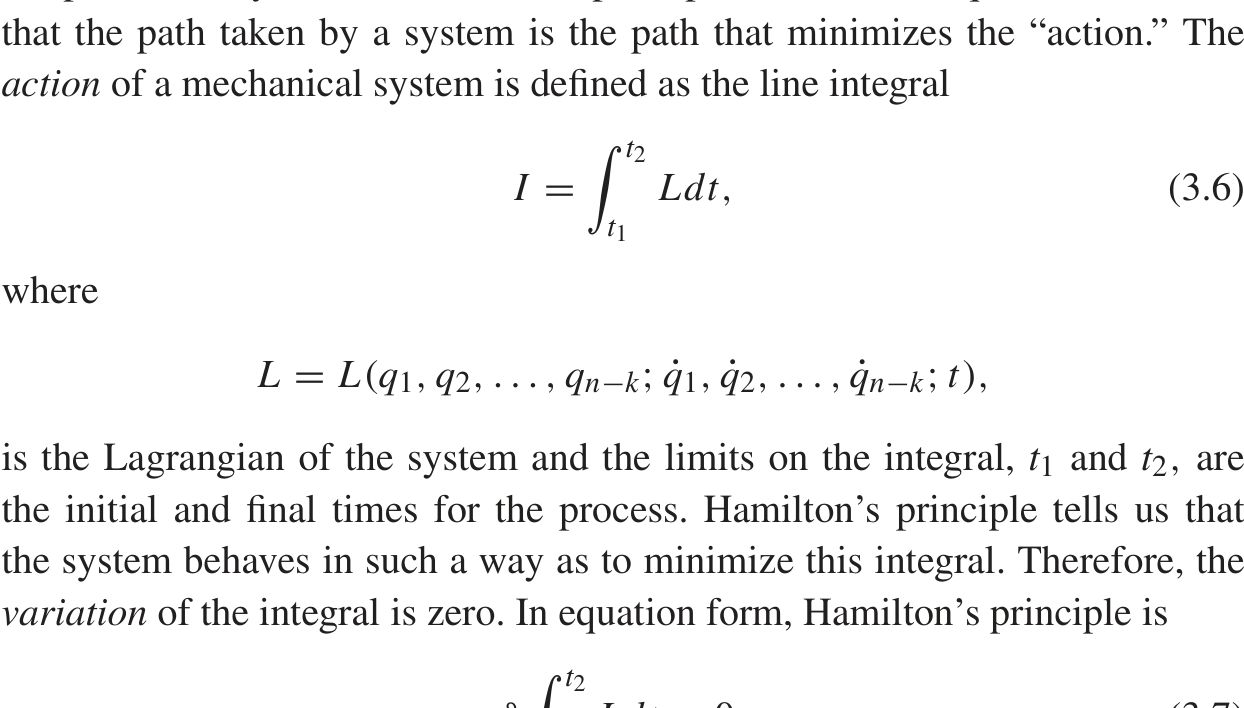
\includegraphics[width=0.55\linewidth]{../Figures/fig_3_1.png}
\caption{Figure 3.1}
\end{figure}

Initial point
Final point
f
Three paths in configuration space.

3.4
Generalization to many coordinates
paths between the end points i and f. Assume that one of these paths is the
one that minimizes the action. (It is the ``true'' path.) Then, along that path,
\textbackslash{}delta
t2
t1 Ldt = 0. The integral is a minimum for the path the system actually
follows, and along any other path the value of the action will be greater.
3.3 Derivation of Lagrange's equations
We can now derive Lagrange's equations from Hamilton's principle, recognizing that a simple change of variables from (x, y, y′) to L(t, q, $\textbackslash{}dot q$) leads to
the nearly trivial reformulation of Hamilton's principle into the language of
the calculus of variations. Hamilton's principle tells us that a mechanical system will follow a path in configuration space given by q = q(t) such that the
integral
tf
ti
L(t, q, $\textbackslash{}dot q$)dt
is minimized. (Note that here the Lagrangian is to be considered a functional.)
Now if q = q(t) is the minimizing path, then L must satisfy the Euler--
Lagrange equation
dt
\textbackslash{}partial L
\textbackslash{}partial $\textbackslash{}dot q$

-\textbackslash{}partial L
\textbackslash{}partial q = 0.
(3.8)
It is customary to call this equation simply ``Lagrange's'' equation. It can easily
be generalized to systems described by an arbitrary number of generalized
coordinates.
\end{exercise}

\begin{exercise}
Exercise 3.3 Show that Equation (3.7) leads to Equation (3.8). Use the
argument given in Section 2.2 as a guide.
\end{exercise}

\section*{3.4  Generalization to many coordinates}

Consider a system described by the generalized coordinates q1, q2, . . . , qn. We
assume the coordinates are all independent. The Lagrangian for this system is
L(q1, q2, . . . , qn, $\textbackslash{}dot q$1, $\textbackslash{}dot q$2, . . . , $\textbackslash{}dot q$n, t). Our plan is to show that Lagrange's equations in the form
dt
\textbackslash{}partial L
\textbackslash{}partial $\textbackslash{}dot q$i

-\textbackslash{}partial L
\textbackslash{}partial qi
= 0,
i = 1, . . . , n

follow from Hamilton's principle. The derivation is similar to that presented in
Section 2.3.
Recall the definition of the variation of a function. If
f = f (qi, $\textbackslash{}dot q$i, t),
then
\textbackslash{}delta f =


\textbackslash{}partial f
\textbackslash{}partial qi

\textbackslash{}delta qi +
\textbackslash{}partial f
\textbackslash{}partial $\textbackslash{}dot q$i

\textbackslash{}delta  $\textbackslash{}dot q$i

.
Note that in this expression, the time is assumed constant.
Consider again Hamilton's principle in the form of Equation (3.7), which is
\textbackslash{}delta
t2
t1
Ldt = \textbackslash{}delta
t2
t1
L(q1, q2, . . . , qn, $\textbackslash{}dot q$1, $\textbackslash{}dot q$2, . . . , $\textbackslash{}dot q$n, t)dt = 0,
or
\textbackslash{}delta I = 0,
where the action is represented by I, and the integral is taken over the ``path''
actually followed by the physical system. Note that for this path the variation in
the action is zero. However, as before, there are an infinite number of possible
paths between the end points, and we express them in the form
Qi(t) = qi(t) + ϵ\textbackslash{}eta i(t).
In this case, the action can be considered a function of ϵ. The Lagrangian L
is a function of Qi, $\textbackslash{}dot Q\_i and (indirectly) of ϵ. Therefore, the variation of the
action is
\textbackslash{}delta I =
t2
t1
\textbackslash{}delta Ldt =
t2
t1

\textbackslash{}partial L
\textbackslash{}partial Qi
\textbackslash{}delta Qi + \textbackslash{}partial L
\textbackslash{}partial $\textbackslash{}dot Q\_i
\textbackslash{}delta  $\textbackslash{}dot Q\_i

dt.
Noting that Qi and $\textbackslash{}dot Q\_i are functions of ϵ, we write
\textbackslash{}delta I = \textbackslash{}partial I
\textbackslash{}partial ϵ dϵ =
t2
t1

\textbackslash{}partial L
\textbackslash{}partial Qi
\textbackslash{}partial Qi
\textbackslash{}partial ϵ dϵ + \textbackslash{}partial L
\textbackslash{}partial $\textbackslash{}dot Q\_i
\textbackslash{}partial $\textbackslash{}dot Q\_i
\textbackslash{}partial ϵ dϵ

dt.
The second term can be integrated by parts. (Note that the mathematical procedure here is nearly identical to that from Equation (2.6) to Equation (2.7).)

3.5
Constraints and Lagrange's \textbackslash{}lambda -method
We have
t2
t1
\textbackslash{}partial L
\textbackslash{}partial $\textbackslash{}dot Q\_i
\textbackslash{}partial $\textbackslash{}dot Q\_i
\textbackslash{}partial ϵ dϵdt =
t2
t1
\textbackslash{}partial L
\textbackslash{}partial $\textbackslash{}dot Q\_i
\textbackslash{}partial 2Qi
\textbackslash{}partial ϵ\textbackslash{}partial t dtdϵ =
t2
t1
\textbackslash{}partial L
\textbackslash{}partial $\textbackslash{}dot Q\_i
\textbackslash{}partial
\textbackslash{}partial ϵ
\textbackslash{}partial Qi
\textbackslash{}partial t dt

dϵ
= \textbackslash{}partial L
\textbackslash{}partial $\textbackslash{}dot Q\_i
\textbackslash{}partial Qi
\textbackslash{}partial ϵ

t2
t1
-
t2
t1
\textbackslash{}partial Qi
\textbackslash{}partial ϵ
dt
\textbackslash{}partial L
\textbackslash{}partial $\textbackslash{}dot Q\_i
dtdϵ
= -
t2
t1
\textbackslash{}partial Qi
\textbackslash{}partial ϵ
dt
\textbackslash{}partial L
\textbackslash{}partial $\textbackslash{}dot Q\_i
dtdϵ,
where we have used the fact that
\textbackslash{}partial Qi
\textbackslash{}partial ϵ

t2
t1
= 0 because all the curves pass
through the end points.
Consequently,
\textbackslash{}delta I =
t2
t1

\textbackslash{}partial L
\textbackslash{}partial Qi
\textbackslash{}partial Qi
\textbackslash{}partial ϵ -\textbackslash{}partial Qi
\textbackslash{}partial ϵ
dt
\textbackslash{}partial L
\textbackslash{}partial $\textbackslash{}dot Q\_i

dϵdt
=
t2
t1

\textbackslash{}partial L
\textbackslash{}partial Qi
-d
dt
\textbackslash{}partial L
\textbackslash{}partial $\textbackslash{}dot Q\_i
\textbackslash{}partial Qi
\textbackslash{}partial ϵ dϵdt
=
t2
t1

\textbackslash{}partial L
\textbackslash{}partial Qi
-d
dt
\textbackslash{}partial L
\textbackslash{}partial $\textbackslash{}dot Q\_i

\textbackslash{}delta Qidt.
When ϵ = 0, \textbackslash{}delta I = 0 because I is minimized along the path qi = qi(t). So
[\textbackslash{}delta I]ϵ=0 = 0 =
t2
t1

\textbackslash{}partial L
\textbackslash{}partial qi
-d
dt
\textbackslash{}partial L
\textbackslash{}partial $\textbackslash{}dot q$i

\textbackslash{}delta qidt.
(3.9)
Since the \textbackslash{}delta qis are independent, the only way this expression can be zero is for
all the terms in the parenthesis to be zero. Hence, Lagrange's equations are
proved.
3.5 Constraints and Lagrange's \textbackslash{}lambda -method
We now apply Lagrange's \textbackslash{}lambda -method of Section 2.4.1 to determine the forces
of constraint acting on a system.
Let a system be described by n generalized coordinates q1, q2, . . . , qn.
Assume, further, that the system is subjected to k holonomic constraints, so
there are k equations relating the coordinates. Obviously, not all of the generalized coordinates are independent, so we could use the k equations of constraint
to reduce the number of generalized coordinates to n -k. However, we prefer,
for the moment, to use all n of the coordinates.

The behavior of the system is described by Hamilton's principle,
\textbackslash{}delta I = \textbackslash{}delta
t2
t1
Ldt = 0,
and the k equations of constraint
fj(q1, q2, . . . , qn) = 0,
j = 1, . . . , k.
(3.10)
If all the coordinates were independent, Hamilton's principle would lead to n
equations of the form
dt
\textbackslash{}partial L
\textbackslash{}partial $\textbackslash{}dot q$i

-\textbackslash{}partial L
\textbackslash{}partial qi
= 0,
i = 1, . . . , n.
(3.11)
But we cannot write this (yet) because as noted following Equation (3.9), this
result depends on all the \textbackslash{}delta qs being independent.
Equations (3.10) represent holonomic constraints. Consequently
\textbackslash{}delta fj = \textbackslash{}partial fj
\textbackslash{}partial q1
\textbackslash{}delta q1 + \textbackslash{}partial fj
\textbackslash{}partial q2
\textbackslash{}delta q2 + \textbackslash{}cdot  \textbackslash{}cdot  \textbackslash{}cdot  + \textbackslash{}partial fj
\textbackslash{}partial qn
\textbackslash{}delta qn = 0.
That is,
n

i=1
\textbackslash{}partial fj
\textbackslash{}partial qi
\textbackslash{}delta qi = 0
j = 1, . . . , k.
(3.12)
Here the coefficients \textbackslash{}partial fj/\textbackslash{}partial qi are functions of the qi. If Equation (3.12) holds,
then multiplying it by some quantity, call it \textbackslash{}lambda j, will have no effect, so we can
write it as
\textbackslash{}lambda j
n

i=1
\textbackslash{}partial fj
\textbackslash{}partial qi
\textbackslash{}delta qi = 0.
The \textbackslash{}lambda s are undetermined multipliers. There are k such equations and adding
them together still yields zero, so
k

j=1
\textbackslash{}lambda j
n

i=1
\textbackslash{}partial fj
\textbackslash{}partial qi
\textbackslash{}delta qi = 0.
Further, we can integrate from ti to tf and still not change the fact that the
value is zero. This yields the useful relation
t2
t1
dt
⎛
⎝
k

j=1
\textbackslash{}lambda j
n

i=1
\textbackslash{}partial fj
\textbackslash{}partial qi
\textbackslash{}delta qi
⎞
⎠= 0.
(3.13)

3.5
Constraints and Lagrange's \textbackslash{}lambda -method
Equation (3.9) can be written as
t2
t1
dt

\textbackslash{}partial L
\textbackslash{}partial qi
-d
dt
\textbackslash{}partial L
\textbackslash{}partial $\textbackslash{}dot q$i

\textbackslash{}delta qi = 0.
(3.14)
Adding Equations (3.13) and (3.14) we obtain
t2
t1
dt

⎛
⎝\textbackslash{}partial L
\textbackslash{}partial qi
-d
dt
\textbackslash{}partial L
\textbackslash{}partial $\textbackslash{}dot q$i
+
k

j=1
\textbackslash{}lambda j
\textbackslash{}partial fj
\textbackslash{}partial qi
⎞
⎠\textbackslash{}delta qi = 0.
(3.15)
The \textbackslash{}delta qs are not all independent; they are related by the k equations of constraint. However, n -k of them are independent and for these coordinates the
term in parenthesis in Equation (3.15) must be zero. For the remaining k equations we can select the undetermined multipliers \textbackslash{}lambda j such that
\textbackslash{}partial L
\textbackslash{}partial qi
-d
dt
\textbackslash{}partial L
\textbackslash{}partial $\textbackslash{}dot q$i
+
k

j=1
\textbackslash{}lambda j
\textbackslash{}partial fj
\textbackslash{}partial qi
= 0.
Consequently, we have, for all qis, the following relations
dt
\textbackslash{}partial L
\textbackslash{}partial $\textbackslash{}dot q$i
-\textbackslash{}partial L
\textbackslash{}partial qi
=
k

j=1
\textbackslash{}lambda j
\textbackslash{}partial fj
\textbackslash{}partial qi
,
i = 1, . . . , n.
(3.16)
Equations (3.16) are n equations and Equations (3.10) give us k equations so
we have n + k equations which can be solved to obtain expressions for the qs
and for the \textbackslash{}lambda s.
We now show how the \textbackslash{}lambda s are related to the generalized forces of constraint.
Consider Lagrange's equations written in the Nielsen form (Equation (3.4)).
Let us write the equation in the following way, in which we separate the conservative forces Qc
i derivable from a potential function (V ) from the forces
of constraint Qnc
(which in general cannot be derived from a potential that
depends only on the coordinates):
dt
\textbackslash{}partial T
\textbackslash{}partial $\textbackslash{}dot q$i
-\textbackslash{}partial T
\textbackslash{}partial qi
= Qc
i + Qnc
i .
The conservative force (Qc) can be expressed as -\textbackslash{}partial V
\textbackslash{}partial qi . Assuming that
\textbackslash{}partial V/\textbackslash{}partial $\textbackslash{}dot q$i = 0, we can write this equation as
dt
\textbackslash{}partial L
\textbackslash{}partial $\textbackslash{}dot q$i
-\textbackslash{}partial L
\textbackslash{}partial qi
= Qnc
i .
(3.17)

a
q
R
s
A disk rolling without slipping on an inclined plane.
But Equations (3.16) and (3.17) must be identical. Hence we have the following expression
Qnc
=
k

j=1
\textbackslash{}lambda j
\textbackslash{}partial fj
\textbackslash{}partial qi
,
and we have obtained the desired expression for the forces of constraint.
\begin{example}
Example 3.1 Consider a disk of radius R rolling down an inclined plane of
length l and angle \textbackslash{}alpha . Find the equations of motion, the angular acceleration,
\begin{figure}[h]
\centering
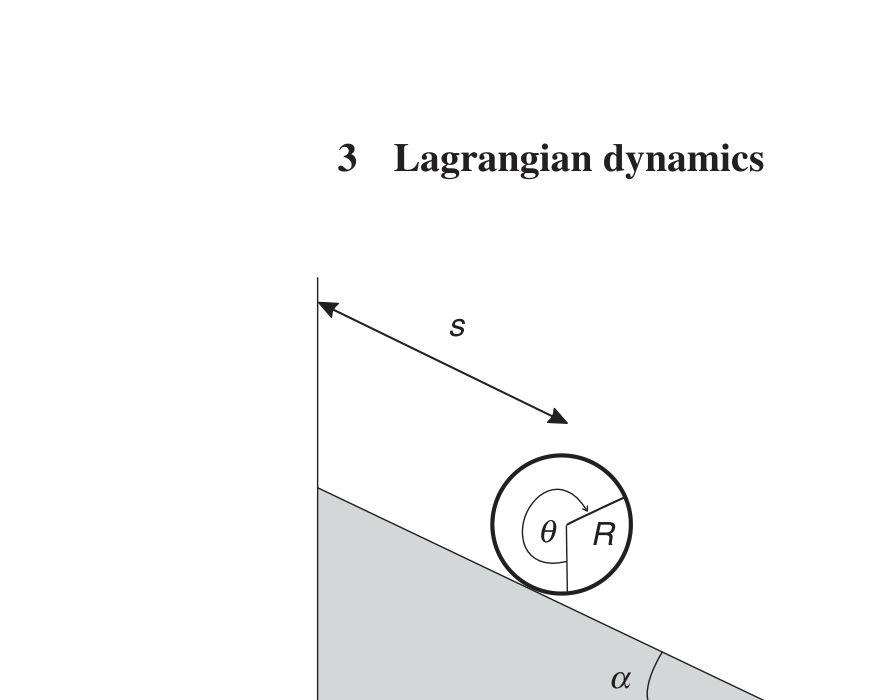
\includegraphics[width=0.55\linewidth]{../Figures/fig_3_2.png}
\caption{Figure 3.2}
\end{figure}

Solution 3.1 The moment of inertia of a disk is I = 1
2MR2, and the kinetic
energy is T = 1
2M $\textbackslash{}dot s$2 + 1
2I $\textbackslash{}dot\textbackslash{}$theta 2. The potential energy is V = Mg(l -s) sin \textbackslash{}alpha .
Therefore,
L = 1
2M $\textbackslash{}dot s$2 + 1
4MR2 $\textbackslash{}dot\textbackslash{}$theta 2 + Mg(s -l) sin \textbackslash{}alpha .
The disk is constrained to roll without slipping. Therefore,
f (s, \textbackslash{}theta ) = s -R\textbackslash{}theta  = 0.
This is a holonomic constraint. Consequently,
dt
\textbackslash{}partial L
\textbackslash{}partial $\textbackslash{}dot s$ -\textbackslash{}partial L
\textbackslash{}partial s = \textbackslash{}lambda \textbackslash{}partial f
\textbackslash{}partial s
where
\textbackslash{}partial f
\textbackslash{}partial s = 1,
dt
\textbackslash{}partial L
\textbackslash{}partial $\textbackslash{}dot\textbackslash{}$theta  -\textbackslash{}partial L
\textbackslash{}partial \textbackslash{}theta  = \textbackslash{}lambda \textbackslash{}partial f
\textbackslash{}partial \textbackslash{}theta
where
\textbackslash{}partial f
\textbackslash{}partial \textbackslash{}theta  = -R.

3.6
Non-holonomic constraints
Carrying out the indicated operations we obtain the two equations of motion
dt (M $\textbackslash{}dot s$) -Mg sin \textbackslash{}alpha  = \textbackslash{}lambda ,
dt
2MR2 $\textbackslash{}dot\textbackslash{}$theta 2

= -R\textbackslash{}lambda .
Furthermore, from the constraint equation we obtain one more equation,
namely,
$\textbackslash{}ddot \textbackslash{}theta$  = $\textbackslash{}ddot s$/R.
You can easily show that
$\textbackslash{}ddot \textbackslash{}theta$  = 2
g sin \textbackslash{}alpha
R
,
and
$\textbackslash{}ddot s$ = 2
3g sin \textbackslash{}alpha .
It follows that
\textbackslash{}lambda  = M $\textbackslash{}ddot s$ -Mg sin \textbackslash{}alpha  = -1
3Mg sin \textbackslash{}alpha .
Now the forces of constraint are given by
Qs = \textbackslash{}lambda \textbackslash{}partial f
\textbackslash{}partial s = -1
3Mg sin \textbackslash{}alpha  = normal force,
and
Q\textbackslash{}theta  = \textbackslash{}lambda \textbackslash{}partial f
\textbackslash{}partial \textbackslash{}theta  = 1
3MgR sin \textbackslash{}alpha  = torque.
Qs and Q\textbackslash{}theta  are the generalized forces required to keep the disk rolling down
the plane without slipping.
\end{example}

\begin{exercise}
Exercise 3.4 Fill in the missing steps in the example above to show that
$\textbackslash{}ddot \textbackslash{}theta$  = (2/3)g sin \textbackslash{}alpha /R and $\textbackslash{}ddot s$ = (2/3)g sin \textbackslash{}alpha .
\end{exercise}

\section*{3.6  Non-holonomic constraints}

Certain non-holonomic constraints can also be treated by Lagrange's \textbackslash{}lambda -method,
as described in Section 2.4.2. Suppose the non-holonomic constraints are

expressed as relations among the differentials of the coordinates. For example,
if there were only one such constraint, it would be given by
A1dq1 + A2dq2 + \textbackslash{}cdot  \textbackslash{}cdot  \textbackslash{}cdot  + Andqn = 0,
where the As are known functions of the qs. If this relation holds for the dqs,
it will also hold for the \textbackslash{}delta qs, so we can write
A1\textbackslash{}delta q1 + A2\textbackslash{}delta q2 + \textbackslash{}cdot  \textbackslash{}cdot  \textbackslash{}cdot  + An\textbackslash{}delta qn = 0.
(3.18)
But this last expression has the same form as the expression for \textbackslash{}delta f for a holonomic constraint, which we wrote as
\textbackslash{}delta f = \textbackslash{}partial f
\textbackslash{}partial q1
\textbackslash{}delta q1 + \textbackslash{}partial f
\textbackslash{}partial q2
\textbackslash{}delta q2 + \textbackslash{}cdot  \textbackslash{}cdot  \textbackslash{}cdot  + \textbackslash{}partial f
\textbackslash{}partial qn
\textbackslash{}delta qn = 0.
Therefore, we can use exactly the same reasoning as before, simply replacing
the \textbackslash{}partial f
\textbackslash{}partial q s with As. (Note, however, that although the As are known quantities,
they are not partial derivatives of some known function.) Consequently, if our
single non-holonomic constraint can be expressed as in Equation (3.18), the
Lagrange equations are
dt
\textbackslash{}partial L
\textbackslash{}partial $\textbackslash{}dot q$i
-\textbackslash{}partial L
\textbackslash{}partial qi
= \textbackslash{}lambda Ai,
i = 1, 2, . . . , n.
If there is more than one non-holonomic constraint, we need to generalize this
relation. For example, if there are m non-holonomic constraints we will have i
equations of the form
dt
\textbackslash{}partial L
\textbackslash{}partial $\textbackslash{}dot q$i
-\textbackslash{}partial L
\textbackslash{}partial qi
=

k=1
\textbackslash{}lambda kAki
i = 1, 2, . . . , n.
We can even use this technique for time dependent (``rheonomic'') constraints having the form
n
i=1
Akidqi + Bktdt = 0,
k = 1, 2, . . . , m.
Here the coefficients (As and Bs) are, in general, functions of both the coordinates and time. As before, we can replace d with \textbackslash{}delta  and write these constraints
in the form
n
i=1
Aki\textbackslash{}delta qi + Bkt\textbackslash{}delta t = 0,
k = 1, 2, . . . , m.

3.7
Virtual work
The coefficients of \textbackslash{}delta t (the Bs) do not enter into the equation of motion because
time is frozen during the virtual displacements, \textbackslash{}delta qi. Thus the equations of
motion take on the familiar form
dt
\textbackslash{}partial L
\textbackslash{}partial $\textbackslash{}dot q$i
-\textbackslash{}partial L
\textbackslash{}partial qi
=

k=1
\textbackslash{}lambda kAki,
i = 1, 2, . . . , n.
Note, however, that the Bs enter into the relations between the velocities, thus
Ai1 $\textbackslash{}dot q$1 + Ai2 $\textbackslash{}dot q$2 + \textbackslash{}cdot  \textbackslash{}cdot  \textbackslash{}cdot  + Ain $\textbackslash{}dot q$n + Bi = 0,
i = 1, 2, . . . , n.
\section*{3.7  Virtual work}

We now consider the concept of virtual work in more detail than was done in
Section 1.6. A mechanical system will be in equilibrium if and only if the total
virtual work of all the ``impressed'' forces is zero. (Impressed forces are those
applied to the system and do not include forces of constraint.1) The principle
of virtual work for a system in equilibrium is expressed mathematically as
\textbackslash{}delta W =

j
Qj\textbackslash{}delta qj = 0.
Here the virtual displacements \textbackslash{}delta qi satisfy all the constraints. Note that the
principle of virtual work is a variational principle.
It is interesting to contrast the principle of virtual work with the Newtonian
concept of equilibrium. In Newtonian mechanics when a system is in equilibrium, the vector sum of all of the forces acting on it is zero. That is, Newtonian mechanics replaces the constraints by forces. Analytical mechanics, on
the other hand, does away with the reaction forces and only considers the
impressed forces; however, it requires that any virtual displacements satisfy the
constraints on the system. (As we shall see, considering virtual displacements
that violate the constraints allows us to determine the forces of constraint.)
In vector notation the generalized forces are just the components of the
actual forces and the principle of virtual work can be expressed as
F1 \textbackslash{}cdot  \textbackslash{}delta r1 + F2 \textbackslash{}cdot  \textbackslash{}delta r2 + \textbackslash{}cdot  \textbackslash{}cdot  \textbackslash{}cdot  + FN \textbackslash{}cdot  \textbackslash{}delta rN = 0.
In terms of Cartesian coordinates, this is
F1x\textbackslash{}delta x1 + F1y\textbackslash{}delta y1 + \textbackslash{}cdot  \textbackslash{}cdot  \textbackslash{}cdot  + FNz\textbackslash{}delta zN = 0.
1 The forces of constraint are often referred to as ``reaction'' forces.

When written in this form, we appreciate that the scalar products of the forces
and the virtual displacements are all zero. This means that the force Fi is
perpendicular to any allowed displacement of particle i. For a free particle,
all displacements are allowed, so the net force must be zero. For a particle
restricted to a table top, the force must be perpendicular to the table top.
If an equilibrium problem involves constraints, then the equilibrium condition can be determined using the Lagrange \textbackslash{}lambda -method.
We have justified the principle of virtual work, but we have not proved it.
Let us leave it as a postulate. (In fact, it is the only postulate of analytical
mechanics and is applicable to dynamical as well as equilibrium situations.2)
Postulate
The virtual work for a system in equilibrium is zero,
\textbackslash{}delta W = 0.
Since Newtonian dynamics states that the total force on a system in equilibrium is zero, we conclude that the reaction forces are equal and opposite to the
impressed forces. Thus, the postulate can be stated in terms of reaction forces
as follows.
Postulate
The virtual work of any force of reaction is zero for any virtual
displacement that satisfies the constraints on the system.
\begin{exercise}
Exercise 3.5 Assume the impressed force is derivable from a scalar function. Show that the equilibrium state is given by the stationary value of the
potential energy, \textbackslash{}delta V = 0.
3.7.1 Physical interpretation of the Lagrange multipliers
In equilibrium, the virtual work of the impressed forces is zero:
\textbackslash{}delta W = 0.
If the impressed forces can be derived from a potential energy (Fi = -\textbackslash{}partial V/\textbackslash{}partial qi)
then the virtual work is equal to the negative of the variation of the potential
energy because
\textbackslash{}delta W = iFi\textbackslash{}delta qi = -i(\textbackslash{}partial V/\textbackslash{}partial qi)\textbackslash{}delta qi = -\textbackslash{}delta V.
If the physical system is subjected to a holonomic constraint given by
f (q1, . . . , qn) = 0,
2 For a discussion of the postulate, see Lanczos, op. cit. page 76.

3.7
Virtual work
then the Lagrange \textbackslash{}lambda -method requires that
\textbackslash{}delta (L + \textbackslash{}lambda f ) = 0.
(See Equation (2.24).) Since \textbackslash{}lambda  is undetermined, we can just as well use -\textbackslash{}lambda
and define a modified Lagrangian by
L = L -\textbackslash{}lambda f.
Since L = T -V, this is equivalent to defining a modified potential energy
V + \textbackslash{}lambda f. Therefore, \textbackslash{}delta W = 0 is equivalent to
\textbackslash{}delta (V + \textbackslash{}lambda f ) = 0.
If we permit arbitrary variations of the generalized coordinates (not just those
that satisfy the constraint), then reaction forces will act on the system. Consequently, the term \textbackslash{}lambda f can be interpreted as the potential energy related to the
force of constraint. Thus, the $\textbackslash{}xi$ component of the reaction force is
Fi = -\textbackslash{}partial (\textbackslash{}lambda f )
\textbackslash{}partial $\textbackslash{}xi$
= -\textbackslash{}lambda  \textbackslash{}partial f
\textbackslash{}partial $\textbackslash{}xi$
-\textbackslash{}partial \textbackslash{}lambda
\textbackslash{}partial $\textbackslash{}xi$
f.
But f = 0, so
Fi = -\textbackslash{}lambda  \textbackslash{}partial f
\textbackslash{}partial $\textbackslash{}xi$
.
We conclude that a holonomic constraint is maintained by forces that can be
derived from a scalar function.
As we have seen, some non-holonomic constraints can also be dealt with
using the Lagrangian \textbackslash{}lambda -method; however, these forces (friction is an example)
cannot be derived from a scalar function.
\end{exercise}

\begin{example}
Example 3.2 You have probably proved by using calculus (perhaps in a previous mechanics course) that the curve formed by a hanging chain or heavy rope
is a catenary. That problem can also be solved using variational techniques.
The quantity to be minimized is the potential energy, V = V (y). The problem
is to determine y = y(x) subject to the constraint that the length of the chain
is a given constant. In variational terms, we want to determine y = y(x) given
that \textbackslash{}delta V = 0 and subject to the constraint
x2
x1 ds = constant = length = l.
Solution 3.2 The constraint can be expressed as
l =
x2
x1

1 + y′2dx.

The potential energy of a length of chain ds is dV = (dm)gh = \textbackslash{}rho gyds.
Dropping unnecessary constants,
V =
x2
x1
yds =
x2
x1
y

1 + y′2dx.
The Lagrange \textbackslash{}lambda -method leads to
\textbackslash{}delta
x2
x1
(y + \textbackslash{}lambda )

1 + y′2dx = 0.
Determining the equation of the curve is left as an exercises.
\end{example}

\begin{exercise}
Exercise 3.6 The functional in the preceding example does not depend
on x. Reformulate the problem as discussed in Section 2.2.2 and show
that the curve is a catenary.
\end{exercise}

\begin{exercise}
Exercise 3.7 Consider a simple pendulum composed of a mass m constrained by a wire of length l to swing in an arc. Assume r and \textbackslash{}theta  are both
variables. Obtain the Lagrange equations and using the \textbackslash{}lambda -method, determine the tension in the wire. Check by using elementary methods.
\end{exercise}

\section*{3.8  The invariance of the Lagrange equations}

The Lagrange equations are invariant under a point transformation. A point
transformation is a transformation from a set of coordinates q1, q2, . . . , qn to
a set s1, s2, . . . , sn such that for every point Pq in ``q-space'' there corresponds
a point Ps in ``s-space.'' The transformation equations have the form
q1 = q1(s1, s2, . . . , sn, t),
...
qn = qn(s1, s2, . . . , sn, t).
It is not difficult to show that the Lagrange equations are invariant under a point
transformation. (That is, they retain the same form. See Problem 3.3 at the end
of the chapter.) However, it may be somewhat more difficult to appreciate the
significance of this invariance, so let us consider it in more detail.
\begin{figure}[h]
\centering
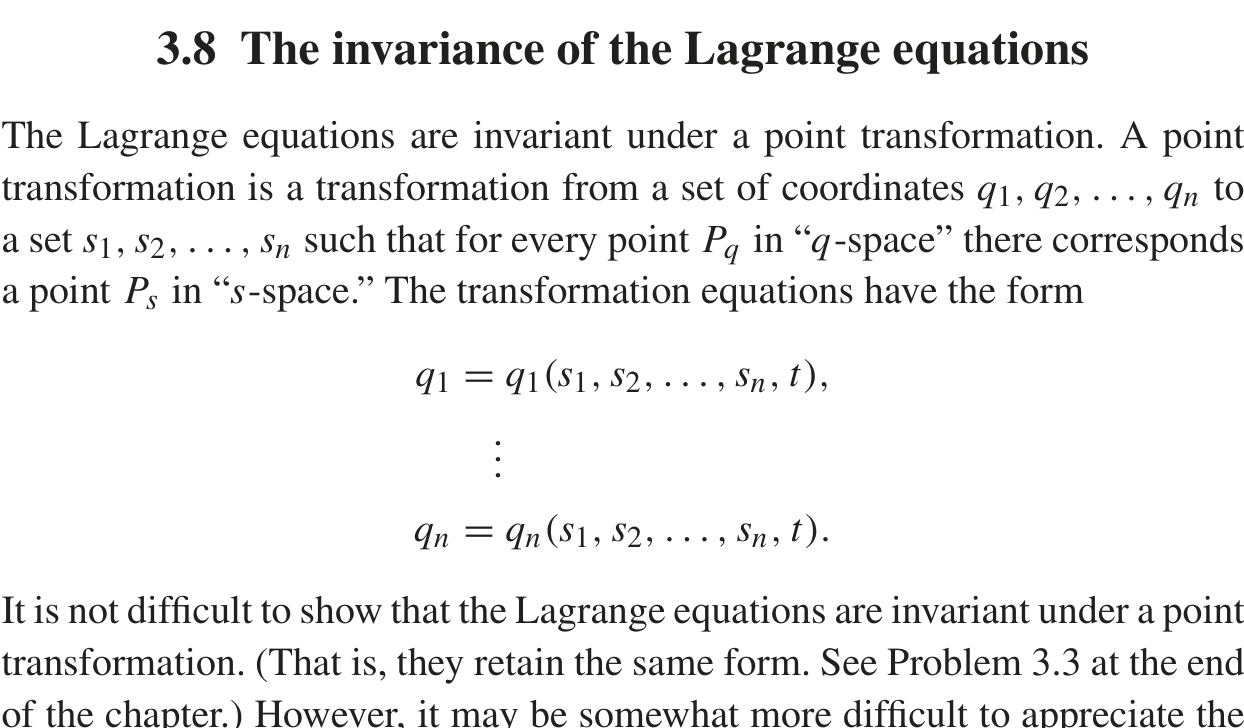
\includegraphics[width=0.55\linewidth]{../Figures/fig_3_3.png}
\caption{Figure 3.3}
\end{figure}

the system is represented by a single point. As time goes on, this point moves

3.8
The invariance of the Lagrange equations
q1
q2
t
s1
s2
t
A
B
A
B
\~{}
\~{}
\~{}
``True'' path in two different coordinate systems.
along a curve.3 The system moves from end point A to end point B along
the curve C that minimizes the action. By considering varied paths between
the same end points and requiring that the action integral be stationary for the
``true'' path, we obtain the conditions
dt
\textbackslash{}partial L
\textbackslash{}partial $\textbackslash{}dot q$i
-\textbackslash{}partial L
\textbackslash{}partial qi
= 0,
i = 1, . . . , n.
Let the coordinates qi be transformed to si by a point transformation. The end
points are transformed to
A,
B and the curve C is transformed to
C, as shown
\begin{figure}[h]
\centering
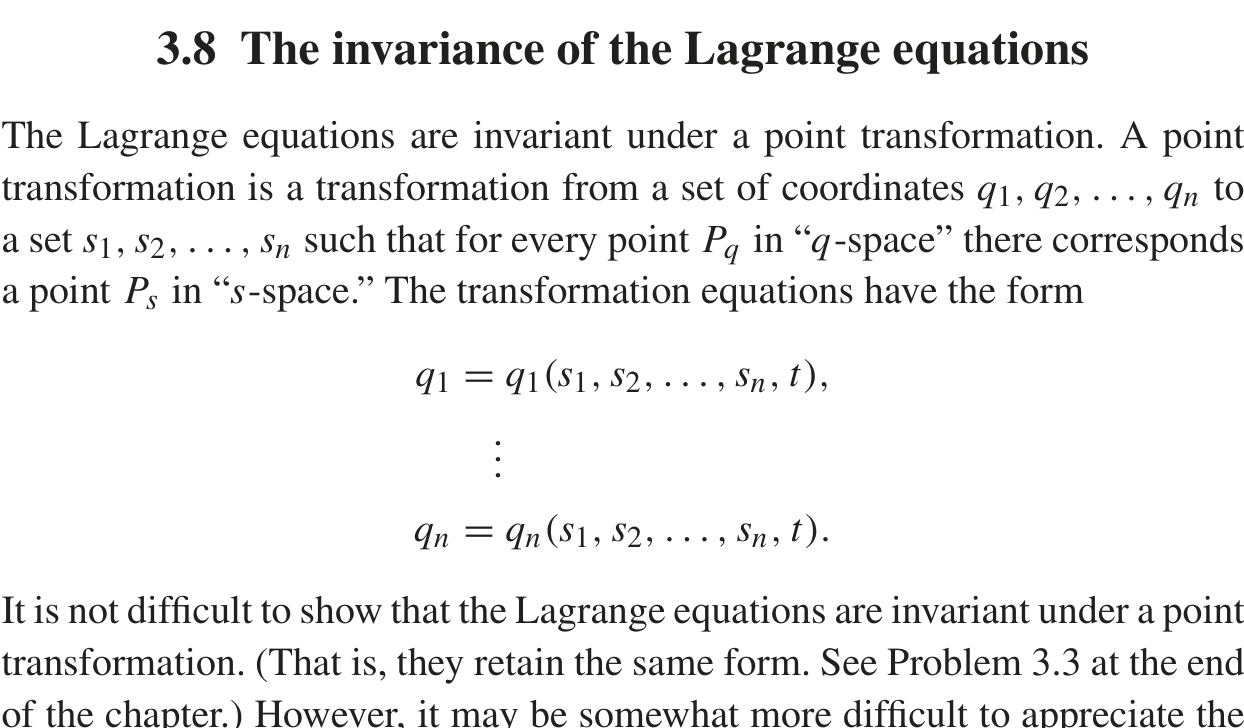
\includegraphics[width=0.55\linewidth]{../Figures/fig_3_3.png}
\caption{Figure 3.3}
\end{figure}

The action integral is minimized by the ``true'' path between the end points
in any coordinate system, consequently the Lagrange equations are valid in the
new coordinate system. Note, however, that although the value of L is the same
in both coordinate system, its form may be quite different. The invariance of
the Lagrange equations allows us to select whatever set of coordinates makes
the equations easiest to solve. (The invariance principle becomes a postulate
in the theory of special relativity in which Einstein postulated that the laws of
physics are invariant under transformations between inertial reference frames.)
The Lagrangian equation of motion for a particular i will not, in general, be
the same in the two systems, but the complete sets of equations are equivalent.
For this reason, one should actually refer to the equations as co-variant rather
than in-variant. For example, if
L = 1
2 $\textbackslash{}dot x$2 + 1
2 $\textbackslash{}dot y$2 +
(x2 + y2)1/2 ,
3 We can include the time as another coordinate, and represent the system as a point in an
(n + 1)-dimensional configuration space. In this space, the system traces out a curve or ``world
line'' that gives the history of the system.

a point transformation, x = r cos \textbackslash{}theta , y = r sin \textbackslash{}theta , yields the Lagrangian
L = 1
2 $\textbackslash{}dot r$2 + 1
2r2 $\textbackslash{}dot\textbackslash{}$theta 2 + 1
r .
The equations of motion in terms of x and y are
$\textbackslash{}ddot x$ = -
(x2 + y2)3
$\textbackslash{}ddot y$ = -
y
(x2 + y2)3 ,
whereas the equations of motion in terms of r and \textbackslash{}theta  are
$\textbackslash{}ddot r$ -r $\textbackslash{}dot\textbackslash{}$theta 2 + 1
r = 0
dt (r2 $\textbackslash{}dot\textbackslash{}$theta ) = 0.
Although these equations of motion are quite different in form, they yield the
same result and for a particular set of the position and velocity parameters they
yield the same numerical value for the Lagrangian.
\section*{3.9  Problems}

\section*{3.1  Assume the generalized force is derivable from a potential independent}

of the generalized velocities. Show that Equations (3.1) follow from Equations (3.4).
3.2 Use d'Alembert's principle to determine the equilibrium condition for
\begin{figure}[h]
\centering
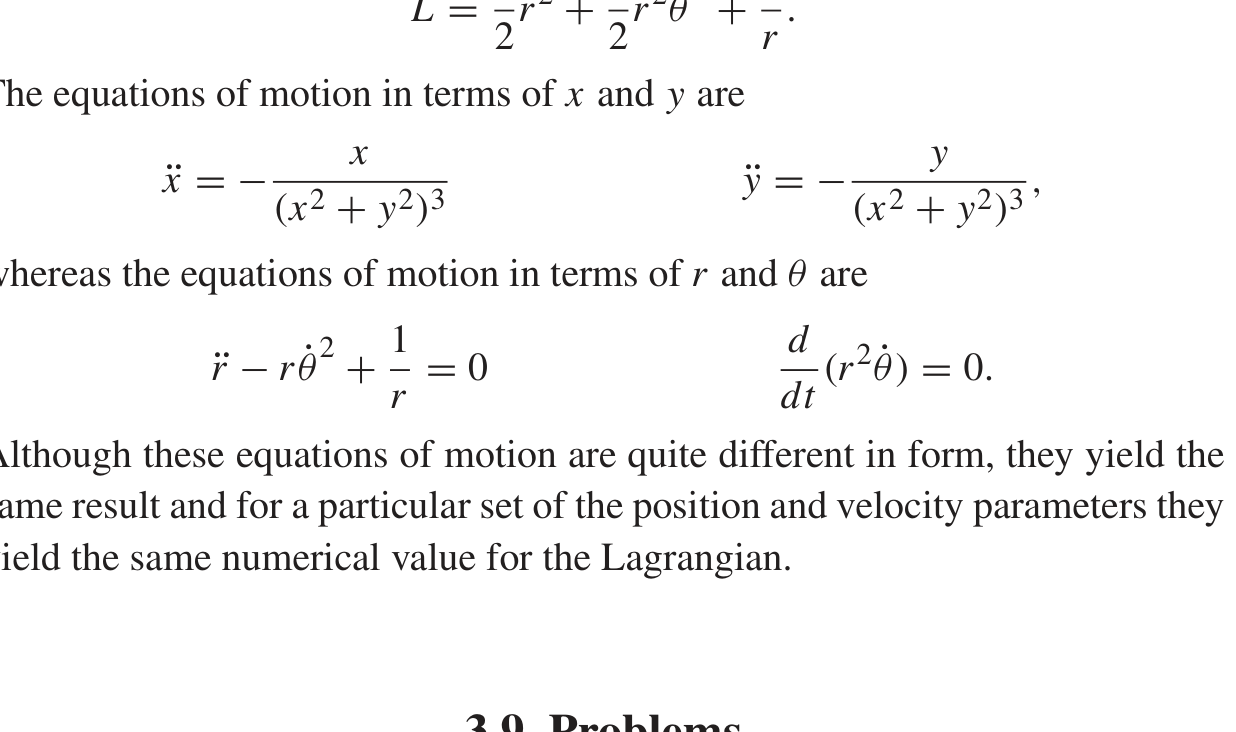
\includegraphics[width=0.55\linewidth]{../Figures/fig_3_4.png}
\caption{Figure 3.4}
\end{figure}

3.3 If one expresses the Lagrangian in terms of some set of generalized coordinates, qi, the Lagrange equations of motion have the form
dt
\textbackslash{}partial L
\textbackslash{}partial $\textbackslash{}dot q$i
-\textbackslash{}partial L
\textbackslash{}partial qi
= 0.
Assume that we transform from the qi to a new set of coordinates si by a
so-called ``point transformation''
qi = qi(s1, s2, . . . , sn, t).
q
f
A system in equilibrium.

3.9
Problems
Prove that Lagrange's equations are unchanged. (That is, prove that
Lagrange's equations are invariant under a point transformation.)
3.4 Consider an object thrown upward in a constant gravitational field.
Demonstrate numerically that
t2
t1 (T -V )dt is smaller for the true path
than for a ``false'' path. Select any ``false'' path you wish.
\section*{3.5  A rope is looped over two frictionless pegs that are at a height h above}

the surface of the Earth and are separated horizontally by a distance d.
The ends of the rope lie on the surface. Determine the equation of the
curve of the hanging portion of the rope.
3.6 A particle slides on the outer surface of an inverted hemisphere. Using
Lagrangian multipliers, determine the reaction force on the particle.
Where does the particle leave the hemispherical surface?
3.7 A right triangular wedge of angle \textbackslash{}theta  and mass M can slide on a frictionless
horizontal surface. A block of mass m is placed on the wedge and it
too can slide on the frictionless inclined surface of the wedge. Use the
method of Lagrange multipliers and determine the equations of motion
for the wedge and the block. Determine the forces of constraint.
\section*{3.8  A particle of mass m1 is connected by an inextensible, massless string}

to a particle of mass m2. Particle m1 is free to slide on the surface of
frictionless table. The string passes through a hole in the table and m2 is
hanging freely under the table and allowed to move only in the vertical
direction. This arrangement will be stable only if m1is moving in a path
around the hole. Write the Lagrangian for the system. Solve the equations
of motion.
3.9 A free body can rotate about any axis. That is,  can have any arbitrary
direction. Consider an allowed displacement of the kth point in the body,
\textbackslash{}delta rk = ϵ \textbackslash{}times  rk.
Using the principle of virtual work, show that this implies the conservation of total angular momentum.
\section*{3.10  According to quantum mechanics, a particle of mass m in a rectangular}

box with sides a, b, c has energy
E = h2
8m
a2 + 1
b2 + 1
c2

.
Assuming the box has constant volume, show that the energy is minimized if the box is a cube (a = b = c).
3.11 Consider a cable of fixed length, suspended from two fixed points. Show
that the shape that minimizes the potential energy is a hyperbolic cosine.

PART II

In this chapter we consider a radically different formulation of the dynamical
problem. We define the Hamiltonian and derive Hamilton's ``canonical'' equations. These are derived in two different ways, first by using a Legendre transformation on the Lagrangian and secondly by using the stationary property of
the action integral. Hamilton's approach gives us a whole new way of looking
at mechanics problems. Although Hamilton's approach is often not as convenient as Lagrange's method for solving practical problems, it is, nevertheless,
a far superior tool for theoretical studies. Some of the methods developed in
Hamiltonian mechanics carry over directly into quantum mechanics, statistical
mechanics, and other fields of physics.
\section*{4.1  The Legendre transformation}

Let us begin by considering the Legendre transformation simply as a mathematical technique. Then (in Section 4.2) we will apply it to the Lagrangian.
The Legendre transformation is useful in a number of branches of physics
and you are probably familiar with it from your thermodynamics course. This
transformation allows us to take a function of one set of variables, such as
f = f (u1, u2, . . . , un),
and generate a new function in terms of the variables vi which are defined by
vi = \textbackslash{}partial f
\textbackslash{}partial ui
.
(4.1)
We shall denote the new function by g, noting that
g = g(v1, v2, . . . , vn).